% This is the Reed College LaTeX thesis template. Most of the work
% for the document class was done by Sam Noble (SN), as well as this
% template. Later comments etc. by Ben Salzberg (BTS). Additional
% restructuring and APA support by Jess Youngberg (JY).
% Your comments and suggestions are more than welcome; please email
% them to cus@reed.edu
%
% See http://web.reed.edu/cis/help/latex.html for help. There are a
% great bunch of help pages there, with notes on
% getting started, bibtex, etc. Go there and read it if you're not
% already familiar with LaTeX.
%
% Any line that starts with a percent symbol is a comment.
% They won't show up in the document, and are useful for notes
% to yourself and explaining commands.
% Commenting also removes a line from the document;
% very handy for troubleshooting problems. -BTS

% As far as I know, this follows the requirements laid out in
% the 2002-2003 Senior Handbook. Ask a librarian to check the
% document before binding. -SN

%%
%% Preamble
%%
% \documentclass{<something>} must begin each LaTeX document
\documentclass[12pt,twoside]{reedthesis}
% Packages are extensions to the basic LaTeX functions. Whatever you
% want to typeset, there is probably a package out there for it.
% Chemistry (chemtex), screenplays, you name it.
% Check out CTAN to see: http://www.ctan.org/
%%
\usepackage{graphicx,latexsym}
\usepackage{amsmath}
\usepackage{amssymb,amsthm}
\usepackage{longtable,booktabs,setspace}
\usepackage{chemarr} %% Useful for one reaction arrow, useless if you're not a chem major
\usepackage[hyphens]{url}
% Added by CII
\usepackage{hyperref}
\usepackage{lmodern}
\usepackage{float}
\floatplacement{figure}{H}
% End of CII addition
\usepackage{rotating}

% Next line commented out by CII
%%% \usepackage{natbib}
% Comment out the natbib line above and uncomment the following two lines to use the new
% biblatex-chicago style, for Chicago A. Also make some changes at the end where the
% bibliography is included.
%\usepackage{biblatex-chicago}
%\bibliography{thesis}


% Added by CII (Thanks, Hadley!)
% Use ref for internal links
\renewcommand{\hyperref}[2][???]{\autoref{#1}}
\def\chapterautorefname{Chapter}
\def\sectionautorefname{Section}
\def\subsectionautorefname{Subsection}
% End of CII addition

% Added by CII
\usepackage{caption}
\captionsetup{width=5in}
% End of CII addition

% \usepackage{times} % other fonts are available like times, bookman, charter, palatino

% Syntax highlighting #22
  \usepackage{color}
  \usepackage{fancyvrb}
  \newcommand{\VerbBar}{|}
  \newcommand{\VERB}{\Verb[commandchars=\\\{\}]}
  \DefineVerbatimEnvironment{Highlighting}{Verbatim}{commandchars=\\\{\}}
  % Add ',fontsize=\small' for more characters per line
  \usepackage{framed}
  \definecolor{shadecolor}{RGB}{248,248,248}
  \newenvironment{Shaded}{\begin{snugshade}}{\end{snugshade}}
  \newcommand{\KeywordTok}[1]{\textcolor[rgb]{0.13,0.29,0.53}{\textbf{#1}}}
  \newcommand{\DataTypeTok}[1]{\textcolor[rgb]{0.13,0.29,0.53}{#1}}
  \newcommand{\DecValTok}[1]{\textcolor[rgb]{0.00,0.00,0.81}{#1}}
  \newcommand{\BaseNTok}[1]{\textcolor[rgb]{0.00,0.00,0.81}{#1}}
  \newcommand{\FloatTok}[1]{\textcolor[rgb]{0.00,0.00,0.81}{#1}}
  \newcommand{\ConstantTok}[1]{\textcolor[rgb]{0.00,0.00,0.00}{#1}}
  \newcommand{\CharTok}[1]{\textcolor[rgb]{0.31,0.60,0.02}{#1}}
  \newcommand{\SpecialCharTok}[1]{\textcolor[rgb]{0.00,0.00,0.00}{#1}}
  \newcommand{\StringTok}[1]{\textcolor[rgb]{0.31,0.60,0.02}{#1}}
  \newcommand{\VerbatimStringTok}[1]{\textcolor[rgb]{0.31,0.60,0.02}{#1}}
  \newcommand{\SpecialStringTok}[1]{\textcolor[rgb]{0.31,0.60,0.02}{#1}}
  \newcommand{\ImportTok}[1]{#1}
  \newcommand{\CommentTok}[1]{\textcolor[rgb]{0.56,0.35,0.01}{\textit{#1}}}
  \newcommand{\DocumentationTok}[1]{\textcolor[rgb]{0.56,0.35,0.01}{\textbf{\textit{#1}}}}
  \newcommand{\AnnotationTok}[1]{\textcolor[rgb]{0.56,0.35,0.01}{\textbf{\textit{#1}}}}
  \newcommand{\CommentVarTok}[1]{\textcolor[rgb]{0.56,0.35,0.01}{\textbf{\textit{#1}}}}
  \newcommand{\OtherTok}[1]{\textcolor[rgb]{0.56,0.35,0.01}{#1}}
  \newcommand{\FunctionTok}[1]{\textcolor[rgb]{0.00,0.00,0.00}{#1}}
  \newcommand{\VariableTok}[1]{\textcolor[rgb]{0.00,0.00,0.00}{#1}}
  \newcommand{\ControlFlowTok}[1]{\textcolor[rgb]{0.13,0.29,0.53}{\textbf{#1}}}
  \newcommand{\OperatorTok}[1]{\textcolor[rgb]{0.81,0.36,0.00}{\textbf{#1}}}
  \newcommand{\BuiltInTok}[1]{#1}
  \newcommand{\ExtensionTok}[1]{#1}
  \newcommand{\PreprocessorTok}[1]{\textcolor[rgb]{0.56,0.35,0.01}{\textit{#1}}}
  \newcommand{\AttributeTok}[1]{\textcolor[rgb]{0.77,0.63,0.00}{#1}}
  \newcommand{\RegionMarkerTok}[1]{#1}
  \newcommand{\InformationTok}[1]{\textcolor[rgb]{0.56,0.35,0.01}{\textbf{\textit{#1}}}}
  \newcommand{\WarningTok}[1]{\textcolor[rgb]{0.56,0.35,0.01}{\textbf{\textit{#1}}}}
  \newcommand{\AlertTok}[1]{\textcolor[rgb]{0.94,0.16,0.16}{#1}}
  \newcommand{\ErrorTok}[1]{\textcolor[rgb]{0.64,0.00,0.00}{\textbf{#1}}}
  \newcommand{\NormalTok}[1]{#1}

% To pass between YAML and LaTeX the dollar signs are added by CII
\title{My Final College Paper}
\author{Charles Jason Tinant}
% The month and year that you submit your FINAL draft TO THE LIBRARY (May or December)
\date{May 2018}
\division{Mathematics and Natural Sciences}
\advisor{Advisor F. Name}
\institution{South Dakota School of Mines and Technology}
\degree{Bachelor of Arts}
%If you have two advisors for some reason, you can use the following
% Uncommented out by CII
% End of CII addition

%%% Remember to use the correct department!
\department{Mathematics}
% if you're writing a thesis in an interdisciplinary major,
% uncomment the line below and change the text as appropriate.
% check the Senior Handbook if unsure.
%\thedivisionof{The Established Interdisciplinary Committee for}
% if you want the approval page to say "Approved for the Committee",
% uncomment the next line
%\approvedforthe{Committee}

% Added by CII
%%% Copied from knitr
%% maxwidth is the original width if it's less than linewidth
%% otherwise use linewidth (to make sure the graphics do not exceed the margin)
\makeatletter
\def\maxwidth{ %
  \ifdim\Gin@nat@width>\linewidth
    \linewidth
  \else
    \Gin@nat@width
  \fi
}
\makeatother

\renewcommand{\contentsname}{Table of Contents}
% End of CII addition

\setlength{\parskip}{0pt}

% Added by CII
  %\setlength{\parskip}{\baselineskip}
  \usepackage[parfill]{parskip}

\providecommand{\tightlist}{%
  \setlength{\itemsep}{0pt}\setlength{\parskip}{0pt}}

\Acknowledgements{
I want to thank a few people.
}

\Dedication{
You can have a dedication here if you wish.
}

\Preface{
This is an example of a thesis setup to use the reed thesis document
class (for LaTeX) and the R bookdown package, in general.
}

\Abstract{
The preface pretty much says it all. \par

Second paragraph of abstract starts here.
}

% End of CII addition
%%
%% End Preamble
%%
%

\usepackage{amsthm}
\newtheorem{theorem}{Theorem}[chapter]
\newtheorem{lemma}{Lemma}[chapter]
\newtheorem{corollary}{Corollary}[chapter]
\newtheorem{proposition}{Proposition}[chapter]
\newtheorem{conjecture}{Conjecture}[chapter]
\theoremstyle{definition}
\newtheorem{definition}{Definition}[chapter]
\theoremstyle{definition}
\newtheorem{example}{Example}[chapter]
\theoremstyle{definition}
\newtheorem{exercise}{Exercise}[chapter]
\theoremstyle{remark}
\newtheorem*{remark}{Remark}
\newtheorem*{solution}{Solution}
\begin{document}

% Everything below added by CII
  \maketitle

\frontmatter % this stuff will be roman-numbered
\pagestyle{empty} % this removes page numbers from the frontmatter
  \begin{acknowledgements}
    I want to thank a few people.
  \end{acknowledgements}
  \begin{preface}
    This is an example of a thesis setup to use the reed thesis document
    class (for LaTeX) and the R bookdown package, in general.
  \end{preface}
  \hypersetup{linkcolor=black}
  \setcounter{tocdepth}{2}
  \tableofcontents

  \listoftables

  \listoffigures
  \begin{abstract}
    The preface pretty much says it all. \par
    
    Second paragraph of abstract starts here.
  \end{abstract}
  \begin{dedication}
    You can have a dedication here if you wish.
  \end{dedication}
\mainmatter % here the regular arabic numbering starts
\pagestyle{fancyplain} % turns page numbering back on

\chapter*{Introduction}\label{introduction}
\addcontentsline{toc}{chapter}{Introduction}

Welcome to the \emph{R Markdown} thesis template. This template is based
on (and in many places copied directly from) the Reed College LaTeX
template, but hopefully it will provide a nicer interface for those that
have never used TeX or LaTeX before. Using \emph{R Markdown} will also
allow you to easily keep track of your analyses in \textbf{R} chunks of
code, with the resulting plots and output included as well. The hope is
this \emph{R Markdown} template gets you in the habit of doing
reproducible research, which benefits you long-term as a researcher, but
also will greatly help anyone that is trying to reproduce or build onto
your results down the road.

Hopefully, you won't have much of a learning period to go through and
you will reap the benefits of a nicely formatted thesis. The use of
LaTeX in combination with \emph{Markdown} is more consistent than the
output of a word processor, much less prone to corruption or crashing,
and the resulting file is smaller than a Word file. While you may have
never had problems using Word in the past, your thesis is likely going
to be about twice as large and complex as anything you've written
before, taxing Word's capabilities. After working with \emph{Markdown}
and \textbf{R} together for a few weeks, we are confident this will be
your reporting style of choice going forward.

\textbf{Why use it?}

\emph{R Markdown} creates a simple and straightforward way to interface
with the beauty of LaTeX. Packages have been written in \textbf{R} to
work directly with LaTeX to produce nicely formatting tables and
paragraphs. In addition to creating a user friendly interface to LaTeX,
\emph{R Markdown} also allows you to read in your data, to analyze it
and to visualize it using \textbf{R} functions, and also to provide the
documentation and commentary on the results of your project. Further, it
allows for \textbf{R} results to be passed inline to the commentary of
your results. You'll see more on this later.

\textbf{Who should use it?}

Anyone who needs to use data analysis, math, tables, a lot of figures,
complex cross-references, or who just cares about the final appearance
of their document should use \emph{R Markdown}. Of particular use should
be anyone in the sciences, but the user-friendly nature of
\emph{Markdown} and its ability to keep track of and easily include
figures, automatically generate a table of contents, index, references,
table of figures, etc. should make it of great benefit to nearly anyone
writing a thesis project.

\hypertarget{rmd-basics}{\chapter{R Markdown Basics}\label{rmd-basics}}

Here is a brief introduction into using \emph{R Markdown}.
\emph{Markdown} is a simple formatting syntax for authoring HTML, PDF,
and MS Word documents. \emph{R Markdown} provides the flexibility of
\emph{Markdown} with the implementation of \textbf{R} input and output.
For more details on using \emph{R Markdown} see
\url{http://rmarkdown.rstudio.com}.

Be careful with your spacing in \emph{Markdown} documents. While
whitespace largely is ignored, it does at times give \emph{Markdown}
signals as to how to proceed. As a habit, try to keep everything left
aligned whenever possible, especially as you type a new paragraph. In
other words, there is no need to indent basic text in the Rmd document
(in fact, it might cause your text to do funny things if you do).

\section{Lists}\label{lists}

It's easy to create a list. It can be unordered like
\begin{itemize}
\tightlist
\item
  Item 1
\item
  Item 2
\end{itemize}
or it can be ordered like
\begin{enumerate}
\def\labelenumi{\arabic{enumi}.}
\tightlist
\item
  Item 1
\item
  Item 2
\end{enumerate}
Notice that I intentionally mislabeled Item 2 as number 4.
\emph{Markdown} automatically figures this out! You can put any numbers
in the list and it will create the list. Check it out below.

To create a sublist, just indent the values a bit (at least four spaces
or a tab). (Here's one case where indentation is key!)
\begin{enumerate}
\def\labelenumi{\arabic{enumi}.}
\tightlist
\item
  Item 1
\item
  Item 2
\item
  Item 3
  \begin{itemize}
  \tightlist
  \item
    Item 3a
  \item
    Item 3b
  \end{itemize}
\end{enumerate}
\section{Line breaks}\label{line-breaks}

Make sure to add white space between lines if you'd like to start a new
paragraph. Look at what happens below in the outputted document if you
don't:

Here is the first sentence. Here is another sentence. Here is the last
sentence to end the paragraph. This should be a new paragraph.

\emph{Now for the correct way:}

Here is the first sentence. Here is another sentence. Here is the last
sentence to end the paragraph.

This should be a new paragraph.

\section{R chunks}\label{r-chunks}

When you click the \textbf{Knit} button above a document will be
generated that includes both content as well as the output of any
embedded \textbf{R} code chunks within the document. You can embed an
\textbf{R} code chunk like this (\texttt{cars} is a built-in \textbf{R}
dataset):
\begin{Shaded}
\begin{Highlighting}[]
\KeywordTok{summary}\NormalTok{(cars)}
\end{Highlighting}
\end{Shaded}
\begin{verbatim}
     speed           dist       
 Min.   : 4.0   Min.   :  2.00  
 1st Qu.:12.0   1st Qu.: 26.00  
 Median :15.0   Median : 36.00  
 Mean   :15.4   Mean   : 42.98  
 3rd Qu.:19.0   3rd Qu.: 56.00  
 Max.   :25.0   Max.   :120.00  
\end{verbatim}
\section{Inline code}\label{inline-code}

If you'd like to put the results of your analysis directly into your
discussion, add inline code like this:
\begin{quote}
The \texttt{cos} of \(2 \pi\) is 1.
\end{quote}
Another example would be the direct calculation of the standard
deviation:
\begin{quote}
The standard deviation of \texttt{speed} in \texttt{cars} is 5.2876444.
\end{quote}
One last neat feature is the use of the \texttt{ifelse} conditional
statement which can be used to output text depending on the result of an
\textbf{R} calculation:
\begin{quote}
The standard deviation is less than 6.
\end{quote}
Note the use of \texttt{\textgreater{}} here, which signifies a
quotation environment that will be indented.

As you see with \texttt{\$2\ \textbackslash{}pi\$} above, mathematics
can be added by surrounding the mathematical text with dollar signs.
More examples of this are in \protect\hyperlink{math-sci}{Mathematics
and Science} if you uncomment the code in
\protect\hyperlink{math}{Math}.

\section{Including plots}\label{including-plots}

You can also embed plots. For example, here is a way to use the base
\textbf{R} graphics package to produce a plot using the built-in
\texttt{pressure} dataset:

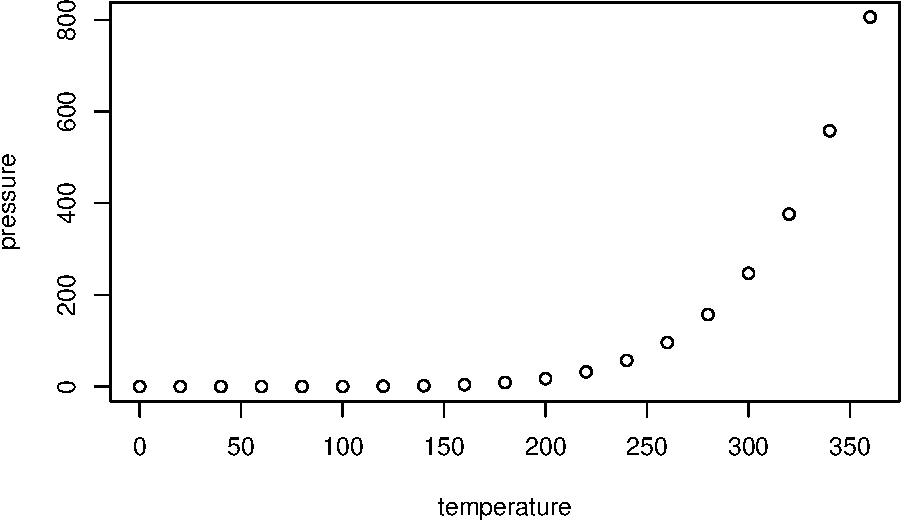
\includegraphics{thesis_files/figure-latex/pressure-1.pdf}

Note that the \texttt{echo=FALSE} parameter was added to the code chunk
to prevent printing of the \textbf{R} code that generated the plot.
There are plenty of other ways to add chunk options. More information is
available at \url{http://yihui.name/knitr/options/}.

Another useful chunk option is the setting of \texttt{cache=TRUE} as you
see here. If document rendering becomes time consuming due to long
computations or plots that are expensive to generate you can use knitr
caching to improve performance. Later in this file, you'll see a way to
reference plots created in \textbf{R} or external figures.

\hypertarget{loading-and-exploring-data}{\section{Loading and exploring
data}\label{loading-and-exploring-data}}

Included in this template is a file called \texttt{flights.csv}. This
file includes a subset of the larger dataset of information about all
flights that departed from Seattle and Portland in 2014. More
information about this dataset and its \textbf{R} package is available
at \url{http://github.com/ismayc/pnwflights14}. This subset includes
only Portland flights and only rows that were complete with no missing
values. Merges were also done with the \texttt{airports} and
\texttt{airlines} data sets in the \texttt{pnwflights14} package to get
more descriptive airport and airline names.

We can load in this data set using the following command:
\begin{Shaded}
\begin{Highlighting}[]
\NormalTok{flights <-}\StringTok{ }\KeywordTok{read.csv}\NormalTok{(}\StringTok{"data/flights.csv"}\NormalTok{)}
\end{Highlighting}
\end{Shaded}
The data is now stored in the data frame called \texttt{flights} in
\textbf{R}. To get a better feel for the variables included in this
dataset we can use a variety of functions. Here we can see the
dimensions (rows by columns) and also the names of the columns.
\begin{Shaded}
\begin{Highlighting}[]
\KeywordTok{dim}\NormalTok{(flights)}
\end{Highlighting}
\end{Shaded}
\begin{verbatim}
[1] 52808    16
\end{verbatim}
\begin{Shaded}
\begin{Highlighting}[]
\KeywordTok{names}\NormalTok{(flights)}
\end{Highlighting}
\end{Shaded}
\begin{verbatim}
 [1] "month"        "day"          "dep_time"     "dep_delay"   
 [5] "arr_time"     "arr_delay"    "carrier"      "tailnum"     
 [9] "flight"       "dest"         "air_time"     "distance"    
[13] "hour"         "minute"       "carrier_name" "dest_name"   
\end{verbatim}
Another good idea is to take a look at the dataset in table form. With
this dataset having more than 50,000 rows, we won't explicitly show the
results of the command here. I recommend you enter the command into the
Console \textbf{\emph{after}} you have run the \textbf{R} chunks above
to load the data into \textbf{R}.
\begin{Shaded}
\begin{Highlighting}[]
\KeywordTok{View}\NormalTok{(flights)}
\end{Highlighting}
\end{Shaded}
While not required, it is highly recommended you use the \texttt{dplyr}
package to manipulate and summarize your data set as needed. It uses a
syntax that is easy to understand using chaining operations. Below I've
created a few examples of using \texttt{dplyr} to get information about
the Portland flights in 2014. You will also see the use of the
\texttt{ggplot2} package, which produces beautiful, high-quality
academic visuals.

We begin by checking to ensure that needed packages are installed and
then we load them into our current working environment:
\begin{Shaded}
\begin{Highlighting}[]
\CommentTok{# List of packages required for this analysis}
\NormalTok{pkg <-}\StringTok{ }\KeywordTok{c}\NormalTok{(}\StringTok{"dplyr"}\NormalTok{, }\StringTok{"ggplot2"}\NormalTok{, }\StringTok{"knitr"}\NormalTok{, }\StringTok{"bookdown"}\NormalTok{, }\StringTok{"devtools"}\NormalTok{)}
\CommentTok{# Check if packages are not installed and assign the}
\CommentTok{# names of the packages not installed to the variable new.pkg}
\NormalTok{new.pkg <-}\StringTok{ }\NormalTok{pkg[}\OperatorTok{!}\NormalTok{(pkg }\OperatorTok\StringTok{ }\KeywordTok{installed.packages}\NormalTok{())]}
\CommentTok{# If there are any packages in the list that aren't installed,}
\CommentTok{# install them}
\ControlFlowTok{if}\NormalTok{ (}\KeywordTok{length}\NormalTok{(new.pkg))}
  \KeywordTok{install.packages}\NormalTok{(new.pkg, }\DataTypeTok{repos =} \StringTok{"http://cran.rstudio.com"}\NormalTok{)}
\CommentTok{# Load packages (thesisdown will load all of the packages as well)}
\KeywordTok{library}\NormalTok{(thesisdown)}
\end{Highlighting}
\end{Shaded}
\clearpage

The example we show here does the following:
\begin{itemize}
\item
  Selects only the \texttt{carrier\_name} and \texttt{arr\_delay} from
  the \texttt{flights} dataset and then assigns this subset to a new
  variable called \texttt{flights2}.
\item
  Using \texttt{flights2}, we determine the largest arrival delay for
  each of the carriers.
\end{itemize}
\begin{Shaded}
\begin{Highlighting}[]
\NormalTok{flights2 <-}\StringTok{ }\NormalTok{flights }\OperatorTok\StringTok{ }
\StringTok{  }\KeywordTok{select}\NormalTok{(carrier_name, arr_delay)}
\NormalTok{max_delays <-}\StringTok{ }\NormalTok{flights2 }\OperatorTok\StringTok{ }
\StringTok{  }\KeywordTok{group_by}\NormalTok{(carrier_name) }\OperatorTok
\StringTok{  }\KeywordTok{summarize}\NormalTok{(}\DataTypeTok{max_arr_delay =} \KeywordTok{max}\NormalTok{(arr_delay, }\DataTypeTok{na.rm =} \OtherTok{TRUE}\NormalTok{))}
\end{Highlighting}
\end{Shaded}
A useful function in the \texttt{knitr} package for making nice tables
in \emph{R Markdown} is called \texttt{kable}. It is much easier to use
than manually entering values into a table by copying and pasting values
into Excel or LaTeX. This again goes to show how nice reproducible
documents can be! (Note the use of \texttt{results="asis"}, which will
produce the table instead of the code to create the table.) The
\texttt{caption.short} argument is used to include a shorter title to
appear in the List of Tables.
\begin{Shaded}
\begin{Highlighting}[]
\KeywordTok{kable}\NormalTok{(max_delays, }
      \DataTypeTok{col.names =} \KeywordTok{c}\NormalTok{(}\StringTok{"Airline"}\NormalTok{, }\StringTok{"Max Arrival Delay"}\NormalTok{),}
      \DataTypeTok{caption =} \StringTok{"Maximum Delays by Airline"}\NormalTok{,}
      \DataTypeTok{caption.short =} \StringTok{"Max Delays by Airline"}\NormalTok{,}
      \DataTypeTok{longtable =} \OtherTok{TRUE}\NormalTok{,}
      \DataTypeTok{booktabs =} \OtherTok{TRUE}\NormalTok{)}
\end{Highlighting}
\end{Shaded}
\begin{longtable}[t]{lr}
\caption[Max Delays by Airline]{\label{tab:maxdelays}Maximum Delays by Airline}\\
\toprule
Airline & Max Arrival Delay\\
\midrule
Alaska Airlines Inc. & 338\\
American Airlines Inc. & 1539\\
Delta Air Lines Inc. & 651\\
Frontier Airlines Inc. & 575\\
Hawaiian Airlines Inc. & 407\\
\addlinespace
JetBlue Airways & 273\\
SkyWest Airlines Inc. & 421\\
Southwest Airlines Co. & 694\\
United Air Lines Inc. & 472\\
US Airways Inc. & 347\\
Virgin America & 366\\
\bottomrule
\end{longtable}
The last two options make the table a little easier-to-read.

We can further look into the properties of the largest value here for
American Airlines Inc. To do so, we can isolate the row corresponding to
the arrival delay of 1539 minutes for American in our original
\texttt{flights} dataset.
\begin{Shaded}
\begin{Highlighting}[]
\NormalTok{flights }\OperatorTok\StringTok{ }\KeywordTok{filter}\NormalTok{(arr_delay }\OperatorTok{==}\StringTok{ }\DecValTok{1539}\NormalTok{, }
\NormalTok{                  carrier_name }\OperatorTok{==}\StringTok{ "American Airlines Inc."}\NormalTok{) }\OperatorTok
\StringTok{  }\KeywordTok{select}\NormalTok{(}\OperatorTok{-}\KeywordTok{c}\NormalTok{(month, day, carrier, dest_name, hour, }
\NormalTok{            minute, carrier_name, arr_delay))}
\end{Highlighting}
\end{Shaded}
\begin{verbatim}
Warning: package 'bindrcpp' was built under R version 3.4.4
\end{verbatim}
\begin{verbatim}
  dep_time dep_delay arr_time tailnum flight dest air_time distance
1     1403      1553     1934  N595AA   1568  DFW      182     1616
\end{verbatim}
We see that the flight occurred on March 3rd and departed a little after
2 PM on its way to Dallas/Fort Worth. Lastly, we show how we can
visualize the arrival delay of all departing flights from Portland on
March 3rd against time of departure.
\begin{Shaded}
\begin{Highlighting}[]
\NormalTok{flights }\OperatorTok\StringTok{ }\KeywordTok{filter}\NormalTok{(month }\OperatorTok{==}\StringTok{ }\DecValTok{3}\NormalTok{, day }\OperatorTok{==}\StringTok{ }\DecValTok{3}\NormalTok{) }\OperatorTok
\StringTok{  }\KeywordTok{ggplot}\NormalTok{(}\KeywordTok{aes}\NormalTok{(}\DataTypeTok{x =}\NormalTok{ dep_time, }\DataTypeTok{y =}\NormalTok{ arr_delay)) }\OperatorTok{+}\StringTok{ }\KeywordTok{geom_point}\NormalTok{()}
\end{Highlighting}
\end{Shaded}
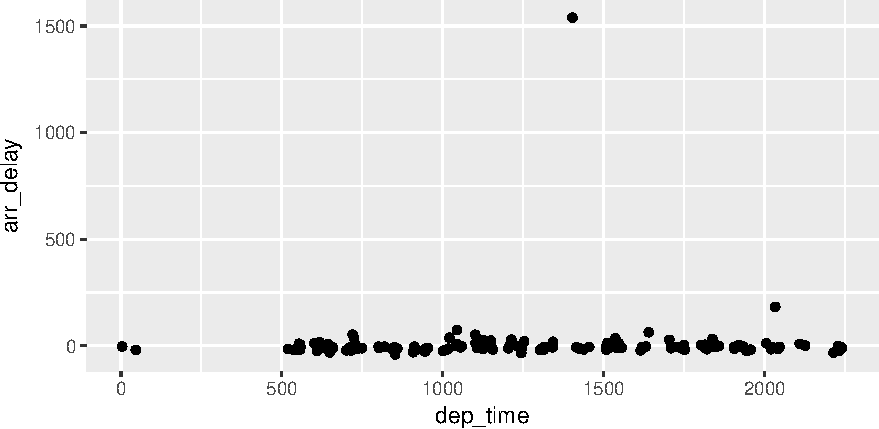
\includegraphics{thesis_files/figure-latex/march3plot-1.pdf}

\section{Additional resources}\label{additional-resources}
\begin{itemize}
\item
  \emph{Markdown} Cheatsheet -
  \url{https://github.com/adam-p/markdown-here/wiki/Markdown-Cheatsheet}
\item
  \emph{R Markdown} Reference Guide -
  \url{https://www.rstudio.com/wp-content/uploads/2015/03/rmarkdown-reference.pdf}
\item
  Introduction to \texttt{dplyr} -
  \url{https://cran.rstudio.com/web/packages/dplyr/vignettes/introduction.html}
\item
  \texttt{ggplot2} Documentation -
  \url{http://docs.ggplot2.org/current/}
\end{itemize}
\section{Overview}\label{overview}

\section{Introduction}\label{introduction-1}

Drought a complex and poorly understood natural hazard that
simultaneously affects many economic sectors and people (Wilhite 2000).
Changing climatic conditions and increases in extreme climate events
have resulted in increased concern about drought frequency, severity,
and duration (Peterson et al. 2013). Drought can be defined as the
extreme persistence of precipitation deficit over a specific region for
a specific period (Zargar et al. 2011). However, a single definition of
drought is not possible because drought effects vary geographically,
temporally, and by economic and environmental sectors impacted by a
reduction in the water supply (Heim 2002). Different drought types are
defined based on the system of interest with operational definitions
used for parts of the hydrologic cycle that experience drought and
conceptual definitions used for societal or ecological systems that
depend on a water supply for which factors outside of the physical
nature of drought exist (Tsakiris and Vangelis 2005).

Drought impacts available water supply to economic and social sectors,
and ecosystems. Socioeconomic drought occurs when water demand is
greater than water supply and results from increased water demand by
growing populations or economic sector development, over-allocation
among competing beneficial uses, or non-sustainable groundwater use
(Frick et al. 1990; Heim 2002; Svoboda and Fuchs 2016). Socioeconomic
drought magnitudes have increased in recent years as a result of the
narrowing of the gap between water supply and water demand (Hayes et al.
2011). Ecological drought is defined as a ``shortage of water causing
stress on ecosystems, adversely affecting the life of plants and
animals'' (Lake 2011). Unlike other forms of drought, ecological drought
does not currently have specific indices to quantify it (Lake 2011;
Svoboda et al. n.d.). The impacts of these types of drought depend on
the magnitude of the water shortage, as well as the vulnerability of a
socioeconomic sector or ecosystem to a reduction in the water supply
(Zargar et al. 2011).

Meteorological, agricultural, and hydrological drought are operationally
defined by duration, magnitude, geographic extent, and frequency, as
well as by drought impacts, indicators, and indices (Wilhite and Glantz
1985; Wilhite et al. 2014; Zargar et al. 2011). Indicators are used in
combination to simplify complex interrelationships these parameters to
derive a drought index. A drought index is a numerical standard based on
water-balance or hydrological models and professional judgment (i.e.,
the US Drought Index) (Svoboda et al. 2015). A drought index objectively
compares cumulative effects of a prolonged and abnormal moisture
deficiency and recurrence probability from region to region and
historical drought to current conditions (Heim 2002; Svoboda and Fuchs
2016; Zargar et al. 2011).

Communication of climate anomalies using drought indices can facilitate
the planning the development of water resources as part of drought risk
management (Wilhite 2000). Duration is the length of a drought, usually
of a minimum of two to three months to become established and continuing
for months to years. Magnitude is the accumulated deficit of water
(e.g., precipitation, soil moisture, or runoff) below some threshold
during a drought period. Drought impact magnitude of drought impacts is
closely related to the timing of the onset of the precipitation
shortage, its intensity, and the duration of the event. Intensity is the
ratio of drought magnitude to duration (Zargar et al. 2011). The degree
of a precipitation shortfall and the severity of associated impacts,
often measured by a departure from expected or average normal
precipitation for a period ranging from one to twelve or more months.
Drought intensity and duration determine the extent of drought impact
(Wilhite 2000). Geographic extent is the areal coverage of the drought
which is variable during the event (Zargar et al. 2011). Drought
frequency or average return period is defined as the average time
between drought events that have a severity that is equal to or greater
than a threshold (Zargar et al. 2011). Drought impacts are defined as an
observable loss or change at a specific time because of drought. Along
with precipitation deficit, drought indicators are combinations of
climate parameters: evapotranspiration, temperature, streamflow,
groundwater and reservoir levels, soil moisture and snowpack (Svoboda
and Fuchs 2016).

Meteorological drought is an extended precipitation deficit over an
extended period between the actual depth of precipitation received and
the expected precipitation depth (Heim 2002). Meteorological drought,
which can develop quickly and end abruptly, leads to other types of
drought. Agricultural drought can rapidly follow a meteorological
drought, particularly during a period of high temperatures and windy
conditions (Heim 2002; Wilhite 2000). Agricultural drought, defined by
sustained soil moisture deficits, leads to low recharge from the soil to
surface and ground waters and may result in hydrological drought.

Agricultural drought ``is typically defined as a period when soil
moisture is inadequate to meet evapotranspiration demands to initiate
and sustain crop growth'' (Changnon 1987). Soil moisture availability is
the difference between actual and potential evapotranspiration (Tate and
Gustard 2000). The potential evapotranspiration (PET) equals the actual
evapotranspiration (AET) when an adequate supply of moisture in the soil
is available to meet vegetation moisture demands. Otherwise, the actual
evapotranspiration is less than the potential evapotranspiration. While
solar radiation is the dominant factor for evapotranspiration, direct
measurements of solar radiation are often unavailable; and mean daily
temperature, latitude, and time of year are used to approximate PET.
Soil infiltration rates, soil moisture capacity, and the magnitude and
timing of precipitation (Heim 2002; Lake 2011). Wilhite (2000) suggests
an operational definition of agricultural drought by comparing
precipitation to AET to determine the rate of soil water depletion, then
expressing the relationship on soil moisture effects on plant
development.

Hydrological drought emphasizes interactions between the natural
characteristics of meteorological drought and the human activities that
depend on precipitation to provide adequate water supplies to meet
societal and environmental demands (Wilhite et al. 2014). Hydrological
drought is ``a period of abnormally dry weather sufficiently prolonged
for the lack of precipitation to cause a serious hydrological
imbalance'' (AMS Council 2013). A hydrological drought has two
components: surface water drought and groundwater drought, ``with the
latter lagging well behind surface water drought in both commencing and
finishing'' (Bond et al. 2008).

Hydrological drought determination is based on the effects of the
precipitation shortfall on the surface or subsurface water supply,
rather than the magnitude of the precipitation deficiency (Dracup et al.
1980; Wilhite 2000). Antecedent soil moisture and aquifer conditions,
hot temperatures, low relative humidity, and desiccating winds are other
factors that may result in agricultural and hydrological droughts
following a short-term absence of precipitation (Heim 2002). Because
time elapses before precipitation deficiencies become evident as reduced
streamflow, reservoir, and groundwater levels, hydrological drought, is
often out of phase with the occurrence of meteorological and
agricultural drought. A hydrological drought may continue for months or
years beyond the termination of other drought types because of the long
time needed to recharge reservoirs or groundwater (Wilhite 2000).

Hydrological drought designation is often based on streamflow (Heim
2002) because streamflow integrates hydrologic processes at the
watershed level. Streamflow at the watershed level includes direct
runoff from the ground surface to a channel, interflow of water into the
stream channel from saturated soils, and base runoff from groundwater
outflow. Reduced stream flows in upstream segments of a basin may result
in lower reservoir and groundwater levels at downstream locations, even
though meteorological drought does not extend to lower portions. Reduced
streamflow impacts public water supply, hydroelectric power production,
recreation, transportation, and agriculture, leading to conflicts
between upstream and downstream water users (Wilhite 2000).

Quantification of hydrologic drought impacts are further complicated by
multiple and often competing hydrological storage system usages such as
irrigation, recreation, tourism, flood control, hydroelectric power
production, domestic water supply, protection of endangered species, and
ecosystem preservation. Timing between meteorological drought and
hydrological drought depends on watershed storage and recharge rates.
Recovery from a hydrologic drought recovery lags the return to normal
meteorological conditions with a length of the lag related to the
groundwater recharge rate that varies with watershed geology and
vertical connectivity (Wilhite et al. 2014).

Ecological drought is defined as a shortage of water causing stress on
ecosystems, adversely affecting the life of plants and animals (Lake
2011). Drought stress is a ramp disturbance that steadily builds in
strength and spatial extent as water availability declines (Humphries
and Baldwin 2003). While hydrology fundamentally influences ecosystem
dynamics, life history strategies, and diversity patterns in streams
(Schriever et al. 2015), water workers have only recently identified
ecological drought as a disturbance. Stream channel water levels (e.g.,
stream stage) drops during a hydrologic drought leading to a weakening
of lateral connectivity as water recedes from the riparian and littoral
zones and backwaters (Boulton, 2003). Hydrological drought results in a
stage reduction caused by decreased lateral connectivity as waters
recede from the riparian and littoral zones and backwaters, and
groundwater flow. Flow reduction causes several abiotic changes
including reduced organic C, N, and P inputs from the riparian zone,
higher water temperatures caused by reduced riparian shading, high air
temperatures, increased salinity, alkalinity, pH, Mg/Ca ratios, hypoxic
conditions, and decreased water clarity. A stream may become
intermittent later in a hydrologic drought, and in streams with high
particulate organic matter concentrations ``blackwater conditions'' can
increase turbidity (Lake 2011; Russell and Johnson 2007). The abiotic
effects of hydrological drought often result in stream ecosystem
changes, including increases in filamentous algae and decreased
heterotrophic production. The ecologic response depends on the magnitude
of the precipitation drought, streamflow permanence, and ecosystem
resiliency (Bonada et al. 2007; Bond et al. 2008; Humphries and Baldwin
2003; Resh et al. 2013). Several authors have distinguished predictable
seasonal drought, allowing for evolutionary or life history adaptations
to dry periods, from an unpredictable supra-seasonal drought that can
result in abrupt long-term changes in community structure (Boersma et
al. 2014; Bogan et al. 2013; Humphries:2003tna Lake 2011).

States and Tribal entities are required under the federal Clean Water
Act to develop standards for their waters to ensure the protection of
beneficial uses protected. The United States Environmental Protection
Agency (US EPA) consults on a government‐to‐government basis with
federally recognized tribes under the EPA Policy on Consultation and
Coordination with Indian Tribes (US Environmental Protection Agency
1995). As discussed above, the study area is the Pine Ridge reservation
and is under the jurisdiction of the Oglala Sioux Tribe (OST). The OST
currently follows South Dakota surface water quality standards for
waters of the Pine Ridge Reservation (SD Dept Environment and Natural
Resources 2017) for beneficial uses including Warm and Cold Water
Permanent and Semi-Permanent Fisheries, Immersion Recreation, Stock
Watering. States and Tribal Entities are required by the US EPA to adopt
either narrative or numeric criteria to maintain or restore biological
integrity in waters under their jurisdiction (US Environmental
Protection Agency 1995). Biological integrity is defined to mean ``the
capability of supporting and maintaining a balanced, integrated, and
adaptive community of organisms having a composition and diversity
comparable to that of natural habitats of the region'' (US Environmental
Protection Agency 2011).

The US EPA recommends a multiple-stressor approach to identify key
stressors (disturbances) and primarily taxa-based metrics such as
taxa-richness, dominance, the percentage of pollution-sensitive taxa,
and percentage of pollution-tolerant taxa (Karr 1999). ``A perturbation
consists of two parts: the disturbance, and the biotic responses to the
disturbance'' (Lake 2003). Stressors (Bunn and Arthington 2002; Poff and
Zimmerman 2010), can be naturally occurring (floods, droughts,
earthquakes, fires) and human-caused (increased nutrient or sediment
loading, human-induced changes in riparian or channel structure. The OST
has designated a Spiritual Use for surface waters under Tribal
jurisdiction. The Tribe has not identified criteria for the Spiritual
Use designation; however, Tribal Resource Agencies indicate their
interest in developing standards-based criteria describing the desired
biological condition of aquatic communities.

Literature Review The World Meteorological Organization (WMO) recommends
the use of drought indices for measuring meteorological, agricultural
and hydrologic drought magnitudes (Hayes et al. 2011). The recommended
drought indices are the Standardized Precipitation Index (SPI) for
meteorological drought, the Standardized Precipitation
Evapotranspiration Index (SPEI), another soil moisture or water balance
index, or the normalized difference vegetation index (NDVI) for
agricultural drought. The WMO discussed the potential for use of the
streamflow drought index (SDI) but did not come to a consensus on a
single hydrological drought index. The WMO has not developed
recommendations for ecological drought.

Drought monitoring in regions where drought occurs mainly because of
precipitation variability is well-represented by SPI because the index
measures the total precipitation deviation from normal over a monthly or
longer averaging period (Fiorillo and Guadagno 2009; Khan et al. 2008;
Vicente-Serrano and López-Moreno 2005). SPI has a solid theoretical
development, is robust to missing data, and is characteristic of a
moving process (Guttman 1999; Heim 2002; Redmond 2002; Svoboda and Fuchs
2016). SPI index values are normally distributed, uniquely related to
the probability of occurrence and can be used to calculate a running
precipitation deficit to indicate drought duration and intensity
(Tsakiris et al. 2006). Since SPI is normalized, it is comparable across
wetter and drier locations, time periods and scales (Tigkas et al. 2014;
Vicente-Serrano et al. 2012). Different drought types can be identified
by SPI, which is a valuable property of the index because hydrologic
systems (i.e., precipitation, soil moisture, streamflow), and regions
(i.e., headwaters, valley fill, karstic) can respond to drought
conditions at different time scales (Vicente-Serrano and López-Moreno
2005). Heim (2002), and Svoboda and Fuchs (2016) suggest the following
time-steps for SPI calculations for different drought types: one to
three months correspond with meteorological drought, three to six months
correspond with agricultural drought, and time steps of twelve months or
longer correspond with hydrological drought. The SPI requires 20 to 30
years of time series data with additional years of data having more
extreme wet and extreme dry observations resulting in more robust
results (Guttman 1999; Svoboda and Fuchs 2016).

The SPI is a dimensionless index that relates dry and wet periods to
frequency and duration. SPI transforms a long-term precipitation record
to standardized series with an average of zero and a standard deviation
of unity. More negative numbers indicate high intensity and less
probable dry events, and, correspondingly, more positive numbers
indicate high intensity and less probable wet events (Svoboda and Fuchs
2016). I provide the mathematical basis for SPI following
Vicente-Serrano's description fitting observations to the Pearson III
distribution (Vicente-Serrano 2006). McKee's (1993) original method used
a two-parameter gamma distribution with parameters estimated by the
maximum likelihood method; however, Guttman (1999) found Pearson III
distribution provides the better goodness of fit. The probability
density function for a Pearson III distributed variable is expressed as:
f(x)=1/αΓ(β) ((x-γ)/α)\^{}(β-1) e\^{}(-((x-γ)/α) ) where α, β and γ are
the shape, scale and origin parameters, respectively, for precipitation
values x \textgreater{} 0; and (β) is the Gamma function of β. The
Pearson III distribution parameters are obtained from L-moment ratios.
The first L-moment ratio, τ2 = λ2/λ1 is analogous to the coefficient of
variation, and the second and third L-moment ratios, τ3 = λ3/λ2 and τ4 =
λ4/λ2 are analogous to coefficients of skewness and kurtosis,
respectively (Hosking 1990). L- moments are linear combinations of
probability weighted moments (PWM), which can be calculated using the
formulae: λ1 = α0( λ2 = α0 − 2α1( λ3 = α0 −6α1 +6α2 λ4 = α0 −12α1 +30α2
−20α3 so PWM of order s is calculated using: a\_s=1/N
∑\_(i=1)\^{}N▒(〖1-F〗\_i )\^{}s x\_i; F\_i=(i-0.35)/N where xi is the
data from a given precipitation series, Fi is the frequency estimator, i
is the range of observations arranged in rising order, and N is the
number of data points (Vicente-Serrano 2006) If τ3 ≥ 1/3, then τm = 1 −
τ3 and β can be obtained using the formula: β= ((0.36067 τ\_m -
〖0.5967τ\_m〗\^{}2 + 0.25361〖τ\_m〗\^{}3 ))/(1 - 2.78861τ\_m +
2.56096〖τ\_m〗\^{}2 - 0.77045〖τ\_m〗\^{}3 ) If τ3 \textless{} 1/3,
then τm = 3π τ32and β can be obtained using the following expression: β=
((1+0.2906 τ\_m ))/(τ\_m + 0.1882〖τ\_m〗\^{}2 - 0.0442〖τ\_m〗\^{}3 )
a=√(π ) λ\_2 (Γ(β))/(Γ(β + 1/2) ) γ = λ\_1-αβ The probability
distribution function of x given by and are calculated analytically:
F(x)=1/(αΓ(β)) ∫\_y\textsuperscript{x▒〖((x-γ)/α)}(β-1) e\^{}(-((x-γ)/α)
) 〗 Pearson III distribution is not defined for x = 0; however,
precipitation series may include months in which there is no
precipitation. An adapted statistic H(x) can be calculated using the
following formula: H(x) = q + (1 - q)F(x) where q is the probability of
zero precipitation and is calculated as m/n, where n is the total number
of months and m is the number of months with no precipitation. The
cumulative probability H(x), is then transformed to the standard normal
random variable z with mean zero and variance of one. Fortunately, SPI
can be calculated using either a stand-alone package available through
the University of Lincoln Drought Mitigation Center webpage (Svoboda and
Fuchs 2016) or using the SPEI package (Beguería and Vicente-Serrano
2017) in the R statistical programming language (R Core Team 2018).
McKee et al. (1993) state that drought begins at an SPI of zero or less;
however, some researchers choose a drought threshold that is less than
zero, but not quite −1 (Svoboda and Fuchs 2016). The drought event
continues until SPI reaches a value greater than zero. A potential
weakness of the SPI is that the index by itself may not account for a
particular region's overall water balance and water use if different
temperatures occur for similar SPI values (Svoboda and Fuchs 2016).
Drought magnitude is the positive sum of the SPI for each month during
the drought event (Hayes et al. 2007). A composite table of narrative
drought classes is shown below with DI (drought index) indicating SPI
(meteorological drought), SPEI (soil moisture drought), and SDI
(hydrological drought) (Lloyd-Hughes 2002; Tigkas et al. 2014) Table 5:
Drought states, descriptions, index values and frequencies Drought State
Description Criterion Percent frequency 0 Extremely wet DI≤2.0 2.3 0
Very wet 1.5≤DI\textless{}2.0 4.4 0 Moderately wet 1.0≤DI\textless{}1.5
9.2 0 Mildly wet 0≤DI\textless{}1.0 34.1 0 Non-drought DI\textgreater{}0
50.0 1 Mild drought -1.0≤DI\textless{}0 34.1 2 Moderate drought
-1.0≤DI\textless{}-1.5 9.2 3 Severe drought -2.0≤DI\textless{}-1.5 4.4 4
Extreme drought -2.0≤DI 2.3

The Standardized Precipitation Evaporation Index (SPEI) is the preferred
index for the overall water balance and water use of a region, in which
temperature variation is non-stationary, or potential evapotranspiration
(PET) is non-negligible (Svoboda and Fuchs 2016). The SPEI represents
departures in the difference between water availability and the
atmospheric water demand, the ``climate water balance.'' SPEI has been
shown to be more effective than SPI in correlating streamflow deficits,
reservoir storage, and water demand, and therefore, is assumed to
provide a reasonable estimate of soil moisture(Lorenzo-Lacruz et al.
2010; Svoboda and Fuchs 2016). A potential weakness of the SPEI is that
the index requires a serially complete dataset for both temperature and
precipitation (Svoboda and Fuchs 2016). The SPEI algorithm calculates
effective precipitation by subtracting PET from precipitation, with PET
estimated by the Thornwaite (Thornthwaite 1948), Penman-Monteith (PM)
(Walter et al. 2000), or Hargreaves equation (Droogers and Allen 2002;
Hargreaves and Samani 1985). The SPEI is mathematically similar to SPI,
except that the input for the index is effective precipitation (Beguería
et al. 2013; Svoboda and Fuchs 2016); and a log-logistic distribution
provides the better goodness of fit than the gamma distribution in the
estimation of SPEI values (Vicente-Serrano et al. 2010a). I provide
below the mathematical basis for SPI following Beguería et al. (2014);
Vicente-Serrano et al. (2010a, 2010b, 2011, 2012) provide a complete
description of the theory behind the SPEI, the computational details,
and comparisons of SPEI with other drought indicators. The probability
distribution function of a variable D according to a log-logistic
distribution is given by: F(D)={[}1+(α/(D-γ))\^{}β {]}\^{}(-1) where
andrepresent the scale, shape, and location parameters that are
estimated from the sample D, which is the difference between
precipitation and PET. An unbiased plotting estimator based on
probability-weighted moments (Hosking 1986) is the default plotting
position method implemented in the SPEI package in R as: w\_s=1/N
∑\_(i=1)\^{}N▒((□((N-i)/s)) D\_i)/□((N-i)/s)

Nalbantis and Tsakiris (Nalbantis and Tsakiris 2009) derived the
standardized streamflow index (SDI) from the SPI to identify hydrologic
drought. The SDI uses monthly streamflow values and the methods of
normalization associated with SPI for developing a drought index based
upon streamflow data (Svoboda and Fuchs 2016). However, it may be
difficult to select the most appropriate distribution to calculate a
streamflow drought index over a wide area because topography, lithology,
vegetation, and human management may increase flow variability within a
basin and change statistical properties of downstream reaches,
(Vicente-Serrano et al. 2012).

Nalbantis and Tsakiris (2008) defined the Streamflow Drought Index (SDI)
is a hydrological drought index with properties identical to the SPI. I
provide the mathematical basis for SPI following Tigkas (2014). The
cumulative streamflow volume Vi k is calculated from the equation:
V\_(i,k)=∑\emph{(j=1)\^{}3k▒Q}(i,j) i=1,2,⋯; j=1,2,⋯12,k=1,2,3,4 for
monthly streamflow volumes Qi j, in which i denotes the hydrological
year, j the month within that hydrological year (j = 1 for October and j
= 12 for September), and k the reference period, k = 1 for
October-December, k = 2 for October-March, k = 3 for October-June, and k
= 4 for October-September. The Streamflow Drought Index (SDI) is defined
for each reference period k of the i-th hydrological year based on the
cumulative streamflow volumes Vi,k by: 〖SDI〗\emph{(i,k)= (V}(i,k)-V
̅\_k)/s\_k , i=1,2,⋯; k=1,2,3,4 in which Vk and sk are the mean and the
standard deviation of cumulative streamflow volumes of the reference
period k. The resulting index is equal to the standardized streamflow
volume. To reduce skewness and because streamflow tends to be
well-approximated by a Gamma distribution, Nalbantis and Tsarkaris
recommend logarithmic transformation of streamflow volume is before SDI
calculation such that\\
〖SDI〗\emph{(i,k)= (y}(i,k)-y ̅\_k)/s\_(y,k) , i=1,2,⋯; k=1,2,3,4 where
y\_k=lna(V\_(i,k) ), i=1,2,⋯; k=1,2,3,4

Streams are increasingly understood as the central agent at the
interface of the co-evolution of climate, geology, topography and
ecology and their transient and long-term responses to change
(Hrachowitz et al. 2014; Thorp 2014). Hydrological systems respond
differently at various time scales because of lithologic and geometric
watershed differences (Lopez-Moreno et al. 2013). Effective prediction
of streamflow responses to drought is increasingly understood in
managing for sustainable water supply (Vörösmarty et al. 2000) and water
quality (Kundzewicz et al. 2008).\\
Hydrology fundamentally influences ecosystem dynamics, life history
strategies, and diversity patterns in streams (Belmar et al. 2013;
Bonada et al. 2007; Gallart et al. 2012; Ledger et al. 2013a; Lytle and
Poff 2016; Olden and Poff 2003). Differences in streamflow dynamics
result in strong habitat-filters favoring taxa adapted to particular
hydrological extremes as well as habitat generalists capable of
persisting in a variety of habitats (Schriever et al. 2015). Ecological
community composition can remain stable for a long time and rapidly
transition into an alternative stable state (Bogan and Lytle 2011; Bogan
et al. 2015; Yodzis 1989). Hydrologic drought results in a progressive
habitat loss, depletion of food resources, and increased predation and
interspecific competition that puts aquatic biota under stress (Bond et
al. 2008).

Stream biota exhibit a variable response to seasonal and supra-seasonal
drought; tending to exhibit high resistance to seasonal drought, and low
resistance and variable resilience to supra-seasonal drought (Boersma et
al. 2014; Bogan et al. 2015). Native biota in drought-prone systems has
evolved resistance or resilience traits that allow them to survive
predictable drought (Boersma et al. 2014; Lytle and Poff 2016; Robinson
et al. 1992; Stanley et al. 1994; Stubbington et al. 2016), including
flow cessation resulting in \textgreater{}95\% habitat contraction
(Bogan and Lytle 2007). Biota with resistance traits to `sit out the
drought' either possess desiccation resistant life-history stages or
utilize `refugia,' habitats that offer less harsh conditions in an
otherwise drought-affected environment (Adams and Warren 2005;
Arthington et al. 2005; Bond et al. 2008; Stubbington 2012). Biota with
resilience traits have mechanisms allowing widespread and rapid
dispersal among suitable habitat patches (Bond et al. 2008; Boulton
2003; Fritz and Dodds 2004; Humphries and Baldwin 2003). Community
recovery, particularly in perennial streams, tends to be rapid following
seasonal drought, with resilience mechanisms responsible for a greater
portion of recovery (Datry et al. 2014). However, supra-seasonal drought
may cause stream intermittency and community turnover in which
short-lived (\textless{}1 year) strong dispersers replace relatively
long-lived (≥1 year) weak dispersers. The regime shift may delay or
preclude recovery to pre-drought conditions, and potential for community
recovery from extreme drought decreases with greater drought magnitude
and duration, hydrologic connectivity, and proximity to drought refuges
(Bogan et al. 2015; Robson et al. 2011).

A literature review returned some prior work on stream community
alteration and recovery from drought in Great Plains streams. Dodds
(2004) summarized macroinvertebrate recovery in the Great Plains
following drought. He found community composition immediately following
a drought is dominated by taxa with drought-resistant traits with a
general colonization sequence reflecting life-cycle length. Initial
recruitment following a drought is made up of upper-reach drift of
resistant taxa plus resilient taxa, such as chironomid midges, with high
growth and reproduction rates that aerially colonize stream reaches.
Larger invertebrates with slower lifecycles, stoneflies and caddisflies,
tend to arrive one to two months post-drought (Dodds et al. 2004).

Miller and Golladay (1996) investigated effects of seasonal drought the
macroinvertebrate community in an intermittent stream in southeastern
Oklahoma. Invertebrate density in pools doubled during a gradual
five-month summer drying event and increased six-fold during a spring
drying event. The density increase was dominated by biting midges
(ceratopogonids) and nonbiting midges (chironomids) and aquatic worms
(oligochaetes) during both drying events. Small squaregill mayfly
(caenids), which were the major taxon in riffles, density in pools
increased during the spring drying event, but did not increase during
the summer drying event. Post-drought recovery in riffles was first
dominated by black flies (simuliids), until three-months later when
rolled-winged stoneflies (leuctrids) became the most dominant taxon.
Water scavenger (hydrophilid) beetle density did not substantially
change during drought (Miller and Golladay 1996). Research in semi-arid
regions outside the Great Plains (Bêche et al. 2009; Bogan et al. 2015;
Pace et al. 2013), arid regions (Sponseller et al. 2010), and mesocosms
(Ledger et al. 2013a; b) provides other analogs for Pine Ridge
reservation stream community alteration and recovery from drought. Resh,
Bêche, and others (2013) provide general description of the effects of
drought stress in their synthesis of community change in
Mediterranean-climate streams in California. They found severe drought
resulted in macroinvertebrate community shifts, and rapid changes in
age-structure from multi-cohort to single-cohort that recovered slowly
(\textasciitilde{}10 years). Bogan and Lytle (2011) found temperature
and pool area, and conductivity accounted for nearly 90\% of variance as
a stream shifted from perennial to intermittent during a supraseasonal
drought. Pre-drought conditions were characterized by a diverse
low-resilience and long-lived community of skimmer dragonflies
(libellulids), giant water bugs (belostomatids), broad-shouldered water
striders (veliids), and beetles (coleopterans: dryopids, dytiscids,
haliplids). The post supra-seasonal drought community was equally
diverse. However, short-lived vagrile taxa characterized the
post-drought community of baetids, veliids, water striders (gerrids),
diving water beetles (dytiscids), and minute moss-beetles (hydraenids)
(Bogan and Lytle 2011). Bêche and others (2009) used indicator species
analysis to characterize successional communities pre-drought and
following a supra-seasonal (1.3\% recurrence interval) drought. They
found the dominant taxa for the pre-drought period included northern and
mortar-joint casemaker caddisflies (limnephilids and odontocerids),
creeping water beetles (naucorids), and stratiomyids. Post-drought
dominant early successional taxa included hydroptilids, and stratiomyids
followed by mid-successional dytiscids, hydrophilids, and sandflies
(ceratopogonid), and late-successional comb-mouthed mayflies
(ameletids), baetids, and green stoneflies (chloroperlids) became
dominant in late succession. Crane flies (tipulids) were drought
indicators in all successional stages. They concluded there was no
evidence of a complete post-drought community recovery following the
supra-seasonal drought (Bêche et al. 2009) Pace and others (2013)
studied the drought response of mayflies, stoneflies, and caddisflies,
collectively (EPT) in wet- and dry- Mediterranean climate streams in a
Catalonia, Spain between 1995-2008. They found the EPT compositional
shifts from drought were less extensive in the wet mesoclimate streams
that experienced a less-severe drought and had greater baseflow. The EPT
community in wet mesoclimate streams shifted from a pre-drought
community of prong-gilled mayflies (leptophlebiids), chloroperlids, and
nemourids to a post-drought community of baetids, stripetail stoneflies
(perlodids), and saddle casemaker (glossosomatid), limnephilid and
bushtailed (sericostomatid) caddisflies. The EPT community in dry
mesoclimate streams shifted from a pre-drought community of flat-headed
mayflies (heptageniids) and hydropsychids to a post-drought community of
baetids, limnephiloids, hydropsychids, and net-tube caddisflies
(psychomyiids)

Bogan, Boersma and others (2014, 2015) identified drought-intolerant and
drought-tolerant taxa. The seasonal-drought intolerant taxa included
small minnow (baetid) mayflies, small winter (capniid) and spring
(nemourid) stoneflies, net-spinning (hydropsychid) caddisflies, riffle
(elmid) and water-penny (psephenid) beetles, and naucorids. Seasonal
drought-adapted (e.g., resistant) taxa included calamoceratid
caddisflies, diving beetles (dytiscids), giant water bugs
(belostomatids), true flies (dipterans; including ceratopogonids,
chironomids, corydalids, simuliids, stratiomyids and tabanids), and
non-insects (copepods, amphipods, and mites). Instream colonizers
included primitive-minnow (siphlonurid) mayflies, tube-case
(limnephilid) caddisflies, capniids, net-winged midges (blepharicerids).
Drought-resilient early-areal colonizers following seasonal drought
including backswimmer and water-boatman (notonectid and corixid) water
bugs, and diving and water scavenger (dytiscid and hydrophilid) beetles.
Drought-resilient late-areal colonizers included hydroptilids,
spread-winged damselflies (lestids), and drain flies (psychodids).

Bogan and others (2015) describe macroinvertebrate community
trajectories following extreme supra-seasonal droughts as having little
effect on aquatic invertebrate taxon richness, but significantly
altering community composition from a pre-drying community dominated by
relatively large, long-lived and sedentary taxa to smaller,
shorter-lived and highly vagile taxa, including strong aerial dispersers
post-drought. They documented an eight-year (2001-2009) community
transition in an ecologically isolated series of travertine (limestone
springs) pools in south-eastern Arizona. The pre-drought community was
diverse and characterized by long-lived, poor-dispersing, taxa made up
of large-sized water bugs, libellulids, calamoceratid caddisflies; and
mid-sized veliids, whirligig and creeping water beetles (gyrinids and
halipids). The mid-drought community was dominated by mosquito larvae
(culicids). The post-drought community was characterized by
hydrophilids, dytiscids, and veliids. Three common species and three
uncommon species were extirpated from the post-drought community (Bogan
and Lytle 2011), potentially as a result of low resilience (e.g.~low
dispersal from refugea) (Phillipsen et al. 2015). Bogan and others
(2015) synthesized findings from geographically separated semi-arid
harshly intermittent desert mountain streams to update a conceptual
model of post-drought recovery trajectories developed by Boulton (2003)
to include seasonal vs.~supra-seasonal drought. The model predicts that
low isolation streams following a predictable, mild seasonal drought
should exhibit high species richness as lotic and lentic taxa
`time-share' between wet and dry season. Highly isolated streams
following a low severity drought should exhibit reduced species richness
as weak dispersers experience stochastic extirpations. As some sensitive
taxa and weak dispersers disappear in moderately isolated streams
following a moderate severity drought should experience reduced species
richness. Non-isolated streams following a high severity drought should
experience reduced species richness as populations of resistant taxa
recover and colonists from nearby refuges return. Highly isolated
streams experiencing a severe drought should experience substantial
reductions in species as only the most resistant taxa remain (Bogan et
al. 2015).\\
Storey (2016) investigated macroinvertebrate community compositional
differences drought in forested and pasture-land intermittent streams in
New Zealand. Perennial forested streams were dominated by leptophlebiid
and coloburiscid mayflies, Stony-cased (pycnocentrod) and conoesucid
caddisflies, and elmids, with lesser abundances of chironomids, and
austroperlid and gripopterygid stoneflies. Perennial pastureland streams
were similar to perennial forested streams with the addition of higher
abundances of hydroptilids. In contrast, forested and pastureland
intermittent streams were dominated by gastropods, chironomids,
simuliids, and oligachaetes, with lesser abundances of leptophbiid
mayflies, polycentropodid caddisflies, ostracod and cladoceran shrimps.
Oligochaetes, chironomids, and nematodes increased during dry years,
while mayflies, caddisflies and beetles decreased in intermittent
streams, with `weeks of no flow' as the strongest predictor variable.
Sponseller and others (2010) studied macroinvertebrate community
recovery following spring floods from 1983--1999; including a
supra-seasonal 1989-1990 drought in an intermittent desert stream in
Arizona and found antecedent flow conditions were the best predictor of
macroinvertebrate community structural changes. They found baetid,
snail-case caddisfly (helicopsychid), tipulid, and stratiomyid abundance
decreased following drought and recovered during wet periods (e.g.,
drought resilience). Hydropsychids, which were abundant before a
supra-seasonal drought, were extirpated. Gastropod and ceratopogonid
abundance increased during drought, most likely because of their
tolerance to increased water temperature and corresponding hypoxic
conditions. The early colonizers (e.g.~r-selected taxa), chironomids and
ceratopogonids, were dominant in early post-drought successional stages
but were replaced in dominance in later successional phases by more
slowly-growing hydropsychids, helicopsychids, and gastropods.

Ledger and others simulated the effect prolonged drought on the
structure and functioning of complex food webs with a two-year
experiment using stream mesocosms (Ledger et al. 2013b; a). The results
of their experimental study are consistent with the results of field
studies summarized above: drought triggered losses of species,
especially engulfing macropredators and changes in trophic interactions
resulting from top-down food web erosion leading to their partial
collapse. The recurrent drying disturbances resulted in a
macroinvertebrate community shift to transient communities dominated by
relatively few, r-selected (e.g., multivoltine) and smaller-bodied
species (\textgreater{}50\% decline in secondary production), and
functional feeding group increases in gastropod grazers. Compensatory
dynamics sustained total macroinvertebrate densities (e.g., count per
sampling effort), in part through increased amorphous detritus fluxes to
chironomids. Ledger and others found no evidence that drought promoted
trophic generalists over specialists through indirect effects on food
supply. Instead, drought increased physiological stress, with
large-bodied species being most strongly affected, directly increasing
consumer mortality. Similar regime shifts following a supra-seasonal
drought were reported in a UK chalk stream. The drought reduced taxa
richness and abundance, particularly baetids, ephemerellids, small
squaregill mayflies (caenids) hydropsychids, sericostomatids and
leptocerids (Stubbington et al. 2009).

\hypertarget{math-sci}{\chapter{Mathematics and
Science}\label{math-sci}}

\hypertarget{math}{\section{Math}\label{math}}

\TeX~is the best way to typeset mathematics. Donald Knuth designed
\TeX~when he got frustrated at how long it was taking the typesetters to
finish his book, which contained a lot of mathematics. One nice feature
of \emph{R Markdown} is its ability to read LaTeX code directly.

If you are doing a thesis that will involve lots of math, you will want
to read the following section which has been commented out. If you're
not going to use math, skip over or delete this next commented section.

\section{Chemistry 101: Symbols}\label{chemistry-101-symbols}

Chemical formulas will look best if they are not italicized. Get around
math mode's automatic italicizing in LaTeX by using the argument
\texttt{\$\textbackslash{}mathrm\{formula\ here\}\$}, with your formula
inside the curly brackets. (Notice the use of the backticks here which
enclose text that acts as code.)

So, \(\mathrm{Fe_2^{2+}Cr_2O_4}\) is written
\texttt{\$\textbackslash{}mathrm\{Fe\_2\^{}\{2+\}Cr\_2O\_4\}\$}.

\noindent Exponent or Superscript: \(\mathrm{O^-}\)

\noindent Subscript: \(\mathrm{CH_4}\)

To stack numbers or letters as in \(\mathrm{Fe_2^{2+}}\), the subscript
is defined first, and then the superscript is defined.

\noindent Bullet: CuCl \(\bullet\) \(\mathrm{7H_{2}O}\)

\noindent Delta: \(\Delta\)

\noindent Reaction Arrows: \(\longrightarrow\) or
\(\xrightarrow{solution}\)

\noindent Resonance Arrows: \(\leftrightarrow\)

\noindent Reversible Reaction Arrows: \(\rightleftharpoons\)

\subsection{Typesetting reactions}\label{typesetting-reactions}

You may wish to put your reaction in an equation environment, which
means that LaTeX will place the reaction where it fits and will number
the equations for you.
\begin{equation}
  \mathrm{C_6H_{12}O_6  + 6O_2} \longrightarrow \mathrm{6CO_2 + 6H_2O}
  \label{eq:reaction}
\end{equation}
We can reference this combustion of glucose reaction via Equation
\eqref{eq:reaction}.

\subsection{Other examples of
reactions}\label{other-examples-of-reactions}

\(\mathrm{NH_4Cl_{(s)}}\) \(\rightleftharpoons\)
\(\mathrm{NH_{3(g)}+HCl_{(g)}}\)

\noindent \(\mathrm{MeCH_2Br + Mg}\) \(\xrightarrow[below]{above}\)
\(\mathrm{MeCH_2\bullet Mg \bullet Br}\)

\section{Physics}\label{physics}

Many of the symbols you will need can be found on the math page
\url{http://web.reed.edu/cis/help/latex/math.html} and the Comprehensive
LaTeX Symbol Guide
(\url{http://mirror.utexas.edu/ctan/info/symbols/comprehensive/symbols-letter.pdf}).

\section{Biology}\label{biology}

You will probably find the resources at
\url{http://www.lecb.ncifcrf.gov/~toms/latex.html} helpful, particularly
the links to bsts for various journals. You may also be interested in
TeXShade for nucleotide typesetting
(\url{http://homepages.uni-tuebingen.de/beitz/txe.html}). Be sure to
read the proceeding chapter on graphics and tables.

\chapter{Tables, Graphics, References, and Labels}\label{ref-labels}

\section{Tables}\label{tables}

In addition to the tables that can be automatically generated from a
data frame in \textbf{R} that you saw in
\protect\hyperlink{rmd-basics}{R Markdown Basics} using the
\texttt{kable} function, you can also create tables using \emph{pandoc}.
(More information is available at
\url{http://pandoc.org/README.html\#tables}.) This might be useful if
you don't have values specifically stored in \textbf{R}, but you'd like
to display them in table form. Below is an example. Pay careful
attention to the alignment in the table and hyphens to create the rows
and columns.
\begin{longtable}[]{@{}ccc@{}}
\caption{\label{tab:inher} Correlation of Inheritance Factors for Parents
and Child}\tabularnewline
\toprule
\begin{minipage}[b]{0.29\columnwidth}\centering\strut
Factors\strut
\end{minipage} & \begin{minipage}[b]{0.47\columnwidth}\centering\strut
Correlation between Parents \& Child\strut
\end{minipage} & \begin{minipage}[b]{0.16\columnwidth}\centering\strut
Inherited\strut
\end{minipage}\tabularnewline
\midrule
\endfirsthead
\toprule
\begin{minipage}[b]{0.29\columnwidth}\centering\strut
Factors\strut
\end{minipage} & \begin{minipage}[b]{0.47\columnwidth}\centering\strut
Correlation between Parents \& Child\strut
\end{minipage} & \begin{minipage}[b]{0.16\columnwidth}\centering\strut
Inherited\strut
\end{minipage}\tabularnewline
\midrule
\endhead
\begin{minipage}[t]{0.29\columnwidth}\centering\strut
Education\strut
\end{minipage} & \begin{minipage}[t]{0.47\columnwidth}\centering\strut
-0.49\strut
\end{minipage} & \begin{minipage}[t]{0.16\columnwidth}\centering\strut
Yes\strut
\end{minipage}\tabularnewline
\begin{minipage}[t]{0.29\columnwidth}\centering\strut
Socio-Economic Status\strut
\end{minipage} & \begin{minipage}[t]{0.47\columnwidth}\centering\strut
0.28\strut
\end{minipage} & \begin{minipage}[t]{0.16\columnwidth}\centering\strut
Slight\strut
\end{minipage}\tabularnewline
\begin{minipage}[t]{0.29\columnwidth}\centering\strut
Income\strut
\end{minipage} & \begin{minipage}[t]{0.47\columnwidth}\centering\strut
0.08\strut
\end{minipage} & \begin{minipage}[t]{0.16\columnwidth}\centering\strut
No\strut
\end{minipage}\tabularnewline
\begin{minipage}[t]{0.29\columnwidth}\centering\strut
Family Size\strut
\end{minipage} & \begin{minipage}[t]{0.47\columnwidth}\centering\strut
0.18\strut
\end{minipage} & \begin{minipage}[t]{0.16\columnwidth}\centering\strut
Slight\strut
\end{minipage}\tabularnewline
\begin{minipage}[t]{0.29\columnwidth}\centering\strut
Occupational Prestige\strut
\end{minipage} & \begin{minipage}[t]{0.47\columnwidth}\centering\strut
0.21\strut
\end{minipage} & \begin{minipage}[t]{0.16\columnwidth}\centering\strut
Slight\strut
\end{minipage}\tabularnewline
\bottomrule
\end{longtable}
We can also create a link to the table by doing the following: Table
\ref{tab:inher}. If you go back to
\protect\hyperlink{loading-and-exploring-data}{Loading and exploring
data} and look at the \texttt{kable} table, we can create a reference to
this max delays table too: Table \ref{tab:maxdelays}. The addition of
the \texttt{(\textbackslash{}\#tab:inher)} option to the end of the
table caption allows us to then make a reference to Table
\texttt{\textbackslash{}@ref(tab:label)}. Note that this reference could
appear anywhere throughout the document after the table has appeared.

\clearpage

\section{Figures}\label{figures}

If your thesis has a lot of figures, \emph{R Markdown} might behave
better for you than that other word processor. One perk is that it will
automatically number the figures accordingly in each chapter. You'll
also be able to create a label for each figure, add a caption, and then
reference the figure in a way similar to what we saw with tables
earlier. If you label your figures, you can move the figures around and
\emph{R Markdown} will automatically adjust the numbering for you. No
need for you to remember! So that you don't have to get too far into
LaTeX to do this, a couple \textbf{R} functions have been created for
you to assist. You'll see their use below.

In the \textbf{R} chunk below, we will load in a picture stored as
\texttt{reed.jpg} in our main directory. We then give it the caption of
``Reed logo'', the label of ``reedlogo'', and specify that this is a
figure. Make note of the different \textbf{R} chunk options that are
given in the R Markdown file (not shown in the knitted document).
\begin{Shaded}
\begin{Highlighting}[]
\KeywordTok{include_graphics}\NormalTok{(}\DataTypeTok{path =} \StringTok{"figure/reed.jpg"}\NormalTok{)}
\end{Highlighting}
\end{Shaded}
\begin{figure}

\includegraphics[width=3.47in]{figure/reed} \caption{Reed logo}\label{fig:reedlogo}
\end{figure}
Here is a reference to the Reed logo: Figure \ref{fig:reedlogo}. Note
the use of the \texttt{fig:} code here. By naming the \textbf{R} chunk
that contains the figure, we can then reference that figure later as
done in the first sentence here. We can also specify the caption for the
figure via the R chunk option \texttt{fig.cap}.

\clearpage 

Below we will investigate how to save the output of an \textbf{R} plot
and label it in a way similar to that done above. Recall the
\texttt{flights} dataset from Chapter \ref{rmd-basics}. (Note that we've
shown a different way to reference a section or chapter here.) We will
next explore a bar graph with the mean flight departure delays by
airline from Portland for 2014. Note also the use of the \texttt{scale}
parameter which is discussed on the next page.
\begin{Shaded}
\begin{Highlighting}[]
\NormalTok{flights }\OperatorTok\StringTok{ }\KeywordTok{group_by}\NormalTok{(carrier) }\OperatorTok
\StringTok{  }\KeywordTok{summarize}\NormalTok{(}\DataTypeTok{mean_dep_delay =} \KeywordTok{mean}\NormalTok{(dep_delay)) }\OperatorTok
\StringTok{  }\KeywordTok{ggplot}\NormalTok{(}\KeywordTok{aes}\NormalTok{(}\DataTypeTok{x =}\NormalTok{ carrier, }\DataTypeTok{y =}\NormalTok{ mean_dep_delay)) }\OperatorTok{+}
\StringTok{  }\KeywordTok{geom_bar}\NormalTok{(}\DataTypeTok{position =} \StringTok{"identity"}\NormalTok{, }\DataTypeTok{stat =} \StringTok{"identity"}\NormalTok{, }\DataTypeTok{fill =} \StringTok{"red"}\NormalTok{)}
\end{Highlighting}
\end{Shaded}
\begin{figure}
\centering
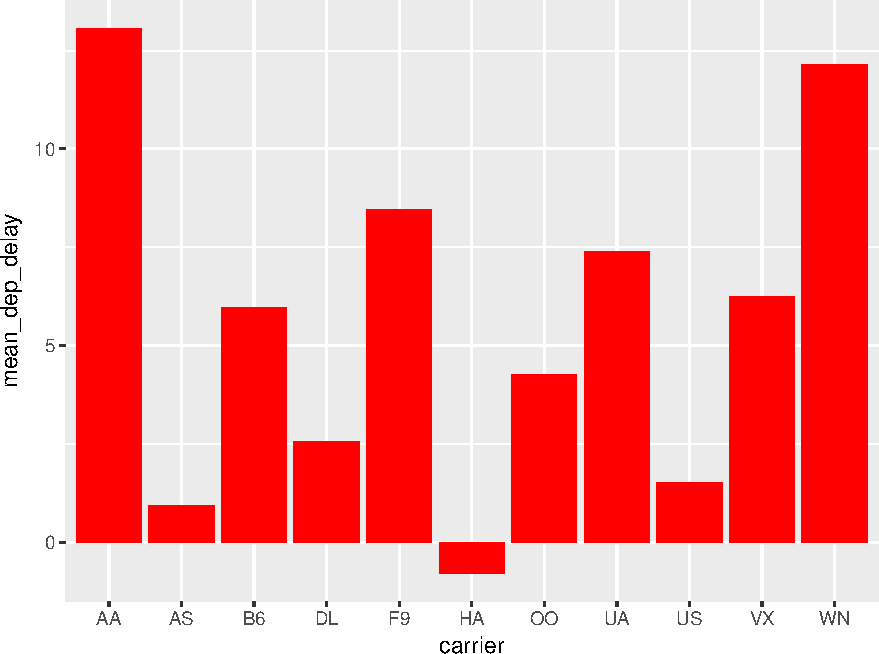
\includegraphics{thesis_files/figure-latex/delaysboxplot-1.pdf}
\caption{\label{fig:delaysboxplot}Mean Delays by Airline}
\end{figure}
Here is a reference to this image: Figure \ref{fig:delaysboxplot}.

A table linking these carrier codes to airline names is available at
\url{https://github.com/ismayc/pnwflights14/blob/master/data/airlines.csv}.

\clearpage

Next, we will explore the use of the \texttt{out.extra} chunk option,
which can be used to shrink or expand an image loaded from a file by
specifying \texttt{"scale=\ "}. Here we use the mathematical graph
stored in the ``subdivision.pdf'' file.
\begin{figure}
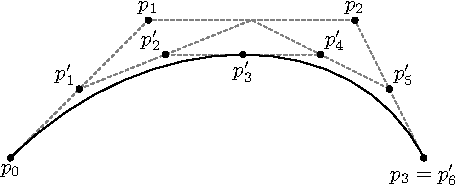
\includegraphics[scale=0.75]{figure/subdivision} \caption{Subdiv. graph}\label{fig:subd}
\end{figure}
Here is a reference to this image: Figure \ref{fig:subd}. Note that
\texttt{echo=FALSE} is specified so that the \textbf{R} code is hidden
in the document.

\textbf{More Figure Stuff}

Lastly, we will explore how to rotate and enlarge figures using the
\texttt{out.extra} chunk option. (Currently this only works in the PDF
version of the book.)
\begin{figure}
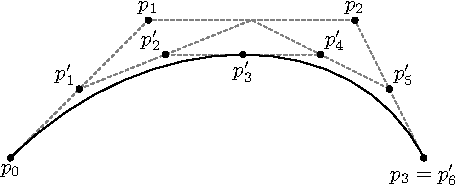
\includegraphics[angle=180, scale=1.1]{figure/subdivision} \caption{A Larger Figure, Flipped Upside Down}\label{fig:subd2}
\end{figure}
As another example, here is a reference: Figure \ref{fig:subd2}.

\section{Footnotes and Endnotes}\label{footnotes-and-endnotes}

You might want to footnote something.\footnote{footnote text} The
footnote will be in a smaller font and placed appropriately. Endnotes
work in much the same way. More information can be found about both on
the CUS site or feel free to reach out to
\href{mailto:data@reed.edu}{\nolinkurl{data@reed.edu}}.

\section{Bibliographies}\label{bibliographies}

Of course you will need to cite things, and you will probably accumulate
an armful of sources. There are a variety of tools available for
creating a bibliography database (stored with the .bib extension). In
addition to BibTeX suggested below, you may want to consider using the
free and easy-to-use tool called Zotero. The Reed librarians have
created Zotero documentation at
\url{http://libguides.reed.edu/citation/zotero}. In addition, a tutorial
is available from Middlebury College at
\url{http://sites.middlebury.edu/zoteromiddlebury/}.

\emph{R Markdown} uses \emph{pandoc} (\url{http://pandoc.org/}) to build
its bibliographies. One nice caveat of this is that you won't have to do
a second compile to load in references as standard LaTeX requires. To
cite references in your thesis (after creating your bibliography
database), place the reference name inside square brackets and precede
it by the ``at'' symbol. For example, here's a reference to a book about
worrying: (Molina \& Borkovec, 1994). This \texttt{Molina1994} entry
appears in a file called \texttt{thesis.bib} in the \texttt{bib} folder.
This bibliography database file was created by a program called BibTeX.
You can call this file something else if you like (look at the YAML
header in the main .Rmd file) and, by default, is to placed in the
\texttt{bib} folder.

For more information about BibTeX and bibliographies, see our CUS site
(\url{http://web.reed.edu/cis/help/latex/index.html})\footnote{Reed~College
  (2007)}. There are three pages on this topic: \emph{bibtex} (which
talks about using BibTeX, at
\url{http://web.reed.edu/cis/help/latex/bibtex.html}),
\emph{bibtexstyles} (about how to find and use the bibliography style
that best suits your needs, at
\url{http://web.reed.edu/cis/help/latex/bibtexstyles.html}) and
\emph{bibman} (which covers how to make and maintain a bibliography by
hand, without BibTeX, at
\url{http://web.reed.edu/cis/help/latex/bibman.html}). The last page
will not be useful unless you have only a few sources.

If you look at the YAML header at the top of the main .Rmd file you can
see that we can specify the style of the bibliography by referencing the
appropriate csl file. You can download a variety of different style
files at \url{https://www.zotero.org/styles}. Make sure to download the
file into the csl folder.

\textbf{Tips for Bibliographies}
\begin{itemize}
\tightlist
\item
  Like with thesis formatting, the sooner you start compiling your
  bibliography for something as large as thesis, the better. Typing in
  source after source is mind-numbing enough; do you really want to do
  it for hours on end in late April? Think of it as procrastination.
\item
  The cite key (a citation's label) needs to be unique from the other
  entries.
\item
  When you have more than one author or editor, you need to separate
  each author's name by the word ``and'' e.g.
  \texttt{Author\ =\ \{Noble,\ Sam\ and\ Youngberg,\ Jessica\},}.
\item
  Bibliographies made using BibTeX (whether manually or using a manager)
  accept LaTeX markup, so you can italicize and add symbols as
  necessary.
\item
  To force capitalization in an article title or where all lowercase is
  generally used, bracket the capital letter in curly braces.
\item
  You can add a Reed Thesis citation\footnote{Noble (2002)} option. The
  best way to do this is to use the phdthesis type of citation, and use
  the optional ``type'' field to enter ``Reed thesis'' or
  ``Undergraduate thesis.''
\end{itemize}
\section{Anything else?}\label{anything-else}

If you'd like to see examples of other things in this template, please
contact the Data @ Reed team (email
\href{mailto:data@reed.edu}{\nolinkurl{data@reed.edu}}) with your
suggestions. We love to see people using \emph{R Markdown} for their
theses, and are happy to help.

\chapter*{Conclusion}\label{conclusion}
\addcontentsline{toc}{chapter}{Conclusion}

If we don't want Conclusion to have a chapter number next to it, we can
add the \texttt{\{-\}} attribute.

\textbf{More info}

And here's some other random info: the first paragraph after a chapter
title or section head \emph{shouldn't be} indented, because indents are
to tell the reader that you're starting a new paragraph. Since that's
obvious after a chapter or section title, proper typesetting doesn't add
an indent there.

\appendix

\chapter{The First Appendix}\label{the-first-appendix}

This first appendix includes all of the R chunks of code that were
hidden throughout the document (using the \texttt{include\ =\ FALSE}
chunk tag) to help with readibility and/or setup.

\textbf{In the main Rmd file}
\begin{Shaded}
\begin{Highlighting}[]
\CommentTok{# This chunk ensures that the thesisdown package is}
\CommentTok{# installed and loaded. This thesisdown package includes}
\CommentTok{# the template files for the thesis.}
\ControlFlowTok{if}\NormalTok{ (}\OperatorTok{!}\KeywordTok{require}\NormalTok{(devtools))}
  \KeywordTok{install.packages}\NormalTok{(}\StringTok{"devtools"}\NormalTok{, }\DataTypeTok{repos =} \StringTok{"http://cran.rstudio.com"}\NormalTok{)}
\ControlFlowTok{if}\NormalTok{ (}\OperatorTok{!}\KeywordTok{require}\NormalTok{(thesisdown))}
\NormalTok{  devtools}\OperatorTok{::}\KeywordTok{install_github}\NormalTok{(}\StringTok{"ismayc/thesisdown"}\NormalTok{)}
\KeywordTok{library}\NormalTok{(thesisdown)}
\end{Highlighting}
\end{Shaded}
\textbf{In Chapter \ref{ref-labels}:}
\begin{Shaded}
\begin{Highlighting}[]
\CommentTok{# This chunk ensures that the thesisdown package is}
\CommentTok{# installed and loaded. This thesisdown package includes}
\CommentTok{# the template files for the thesis and also two functions}
\CommentTok{# used for labeling and referencing}
\ControlFlowTok{if}\NormalTok{(}\OperatorTok{!}\KeywordTok{require}\NormalTok{(devtools))}
  \KeywordTok{install.packages}\NormalTok{(}\StringTok{"devtools"}\NormalTok{, }\DataTypeTok{repos =} \StringTok{"http://cran.rstudio.com"}\NormalTok{)}
\ControlFlowTok{if}\NormalTok{(}\OperatorTok{!}\KeywordTok{require}\NormalTok{(dplyr))}
    \KeywordTok{install.packages}\NormalTok{(}\StringTok{"dplyr"}\NormalTok{, }\DataTypeTok{repos =} \StringTok{"http://cran.rstudio.com"}\NormalTok{)}
\ControlFlowTok{if}\NormalTok{(}\OperatorTok{!}\KeywordTok{require}\NormalTok{(ggplot2))}
    \KeywordTok{install.packages}\NormalTok{(}\StringTok{"ggplot2"}\NormalTok{, }\DataTypeTok{repos =} \StringTok{"http://cran.rstudio.com"}\NormalTok{)}
\ControlFlowTok{if}\NormalTok{(}\OperatorTok{!}\KeywordTok{require}\NormalTok{(ggplot2))}
    \KeywordTok{install.packages}\NormalTok{(}\StringTok{"bookdown"}\NormalTok{, }\DataTypeTok{repos =} \StringTok{"http://cran.rstudio.com"}\NormalTok{)}
\ControlFlowTok{if}\NormalTok{(}\OperatorTok{!}\KeywordTok{require}\NormalTok{(thesisdown))\{}
  \KeywordTok{library}\NormalTok{(devtools)}
\NormalTok{  devtools}\OperatorTok{::}\KeywordTok{install_github}\NormalTok{(}\StringTok{"ismayc/thesisdown"}\NormalTok{)}
\NormalTok{  \}}
\KeywordTok{library}\NormalTok{(thesisdown)}
\NormalTok{flights <-}\StringTok{ }\KeywordTok{read.csv}\NormalTok{(}\StringTok{"data/flights.csv"}\NormalTok{)}
\end{Highlighting}
\end{Shaded}
\chapter{The Second Appendix, for
Fun}\label{the-second-appendix-for-fun}

\backmatter

\chapter*{References}\label{references}
\addcontentsline{toc}{chapter}{References}

\markboth{References}{References}

\noindent

\setlength{\parindent}{-0.20in} \setlength{\leftskip}{0.20in}
\setlength{\parskip}{8pt}

\hypertarget{refs}{}
\hypertarget{ref-angel2000}{}
Angel, E. (2000). \emph{Interactive computer graphics : A top-down
approach with opengl}. Boston, MA: Addison Wesley Longman.

\hypertarget{ref-angel2001}{}
Angel, E. (2001a). \emph{Batch-file computer graphics : A bottom-up
approach with quicktime}. Boston, MA: Wesley Addison Longman.

\hypertarget{ref-angel2002a}{}
Angel, E. (2001b). \emph{Test second book by angel}. Boston, MA: Wesley
Addison Longman.

\hypertarget{ref-Molina1994}{}
Molina, S. T., \& Borkovec, T. D. (1994). The Penn State worry
questionnaire: Psychometric properties and associated characteristics.
In G. C. L. Davey \& F. Tallis (Eds.), \emph{Worrying: Perspectives on
theory, assessment and treatment} (pp. 265--283). New York: Wiley.

\hypertarget{ref-noble2002}{}
Noble, S. G. (2002). \emph{Turning images into simple line-art}
(Undergraduate thesis). Reed College.

\hypertarget{ref-reedweb2007}{}
Reed~College. (2007, March). LaTeX your document. Retrieved from
\url{http://web.reed.edu/cis/help/LaTeX/index.html}


% Index?

\end{document}
